\section{Implementierung}
        
    \subsection{Mobile Applikation}
        
            \subsubsection{Projektaufbau}
        React Native bietet eine Option ein neues Projekt anzulegen. Der Befehl \textit{react-native init <projectname>} generiert alle benötigten Dateien und Ordner, um ein Projekt zu starten. Dies ermöglicht einen schnellen, einfachen Einstieg in React Native. Die initiale Ordnerstruktur wurde im Zuge der React Native Arbeit näher erläutert. Für größere Projekte ist diese Struktur allerdings nicht ideal. Die initial generierten Dateien \textit{index.android.js} und \textit{index.ios.js} dienen den nativen Android und iOS Apps als Ausgangspunkt. Mit dem Befehl \textit{AppRegistry} kann die App dort registriert werden. Die Dateien enthalten zu Anfang allerdings viel doppelten Code. Um die Codequalität zu verbessern und zu vereinheitlichen wurde deshalb die Ordnerstruktur für das Projekt angepasst. Ziele für die Umstrukturierung war die maximale Wiederverwendbarkeit von Code. Listing \ref{lst:directory_structure} zeigt die verwendete Ordnerstruktur.
        
        \lstdefinestyle{tree}{
            literate=
            {├}{{\smash{\raisebox{-1ex}{\rule{1pt}{\baselineskip}}}\raisebox{0.5ex}{\rule{1ex}{1pt}}}}1 
            {─}{{\raisebox{0.5ex}{\rule{1.5ex}{1pt}}}}1 
            {└}{{\smash{\raisebox{0.5ex}{\rule{1pt}{\dimexpr\baselineskip-1.5ex}}}\raisebox{0.5ex}{\rule{1ex}{1pt}}}}1 
        }
        
        \begin{lstlisting}[style=tree]
        .
        ├── .babelrc
        ├── .buckconfig
        ├── .eslintrc.json
        ├── .flowconfig
        ├── .watchmanconfig
        ├── __tests__/
        ├── android/
        ├── app/
        ├── index.android.js
        ├── index.ios.js
        ├── ios/
        ├── node_modules/
        └── package.json
        \end{lstlisting}
        \vspace{-0.5 cm}
        \begin{listing}[H]
            \caption{Verzeichnisstruktur des React Native Projekts}
            \label{lst:directory_structure}
        \end{listing}
        
        Die Android und iOS Ordner enthalten den nativen Code für die Apps. Die React Native Entwicklung der App befindet sich fast ausschließlich in dem Ordner \textit{app}. Die Entwicklung von Tests befindet sich in \textit{\_\_tests\_\_}. Die verwendeten Bibliotheken stehen in der \textit{package.json} Datei und deren Versionen können dort angepasst werden. Die Konfiguration des JavaScript-Compilers befindet sich in der \textit{.babelrc} Datei. Die \textit{package.json} führt die verwendeten Bibliotheken und deren Versionen auf, während die .\textit{eslintrc.json} den Code-Linter konfiguriert.
        
        Im Listing \ref{lst:app_directory_structure} sind die Unterordner des Ordners \textit{app} zu sehen. Die \textit{index.js} Datei wird von den Dateien \textit{index.android.js}und \textit{index.ios.js} importiert. Der erste Ordner ist \textit{components}. Dieser dient der Strukturierung von wiederverwendbaren UI-Komponenten, wie beispielsweise Buttons. \\
        In dem Ordner \textit{config} befinden sich wiederverwendbare Styles, die von mehreren Komponenten genutzt werden. Zusätzlich befinden sich in der \textit{images.js}-Datei Pfade für die verwendeten Bilder. Damit können diese zentral verwaltet werden. Die Bilder selbst werden im Ordner \textit{images} gespeichert.\\
        Die Ordner \textit{database} und \textit{network} enthalten jeweils Module, welche die API-Aufrufe bzw. die Datenbank-Operationen implementieren und über abstrakte Methoden zur Verfügung stellen. \\
        Der \textit{redux}-Ordner beinhaltet die verschiedenen \textit{Actions}, d.h. Events, die den globalen State verändern, sowie die \textit{Reducer}, welche entscheiden, wie eine Action den globalen State verändert.
        
        Die Routen reflektieren die verschiedenen Views in der App. Die Views werden in Kapitel \ref{views} näher erklärt. In dem Ordner \textit{routes} werden die Views implementiert. Hier befindet sich der Hauptteil der Implementierung der App. Die Datei \textit{router.js} ist zuständig für die Navigation zwischen den verschiedenen Views und die gewünschte View anzuzeigen. Die Datei wird von der index.js Datei importiert. Dies sorgt für eine übersichtliche Entwicklung aller Teile der App. 
        
        \begin{lstlisting}[style=tree]
        .
        ├── components
        ├── config
        ├── database
        ├── images
        ├── index.js
        ├── router.js
        ├── network
        ├── redux
        └── routes
        
        \end{lstlisting}
        \vspace{-0.5 cm}
        \begin{listing}[H]
            \caption{Inhalte des Ordners \textit{app}}
            \label{lst:app_directory_structure}
        \end{listing}
    
        \subsubsection{Installation}
Um die React Native Applikation ausführen zu können, muss als erstes Node installiert sein. Zusätzlich sollte \textit{Watchman} installiert werden. Watchman beobachtet Dateiänderungen und sorgt für eine bessere Performance \cite{facebook_inc._start_2017}. Als nächstes kann mit dem Package-Manager \textit{npm} das Paket \textit{react-native-cli} (React Native command line interface) installiert werden. \\

Vor dem Ausführen der App müssen noch die benötigten Libraries installiert werden. Dazu wird im Projektordner folgender Befehl auf dem Terminal aufgerufen:
\begin{listing}[H]
    \begin{minted}{bash}
    npm install
    react-native link
    \end{minted}
    \caption{Installation der benötigten Bibliotheken}
    \label{lst:npm_linstall}
\end{listing}
Zusätzlich sind für die Bibliothek \textit{Image-Crop-Picker } noch einige manuell Schritte nötig. Dieser dient zum auswählen der Bilder in der App. In Xcode muss dafür noch unter \textit{Deployment Info} das \textit{Deployment Target} auf 8.0 gesetzt werden. Unter dem Punkt \textit{Embedded Binaries} werden die beiden Dateien \textit{RSKImageCropper.framework} und \textit{QBImagePicker.framework} noch hinzugefügt \cite{pusic_crop_2017}.

Um die App nun zu starten, sind je nach Zielplattform die in Listing \ref{lst:run} aufgeführten Befehle auszuführen. Dabei ist zu beachten, dass für Android das Android-SDK sowie ein gestarteter Android-Emulator vorhanden sein muss.
\begin{listing}[H]
    \begin{minted}{bash}
    react-native run-ios # Start der App auf dem iPhone-Simulator
    react-native run-android # Stat der App auf dem Android-Simulator
    \end{minted}
    \caption{Ausführen der App}
    \label{lst:run}
\end{listing}

Alternativ kann die App auch über das Xcode-Projekt im \textit{ios}-Ordner der App gestartet werden. Dabei kann eine iOS-App nur auf dem MacOS-System gestartet werden. \cite{facebook_inc._start_2017}\\
Zum Ausführen der Android-App kann außerdem Android Studio oder eine ähnliche Umgebung genutzt werden.

        \subsubsection{Verwendete Bibliotheken}
        
        \subsubsection*{ExNavigation}
Um eine einfache und übersichtliche  Navigation zu gewährleisten wurde die Bibliothek \textit{ExNavigation} verwendet. Die Bibliothek wird im Moment in die reactjs-Organisation eingebunden und daher in der nächsten Version unter dem Namen \textit{react-navigation} verfügbar sein \cite{Vatne_exnavigation_2017}. Die Bibliothek ermöglicht eine einfachere Navigation als die Standard React Native Navigation im Moment. Mit wenig Entwicklungsaufwand konnte so eine einfach zu steuernde Navigation zwischen den Views ermöglicht werden.

        \subsubsection*{Realm}
        Um die vom Nutzer bereitgestellten Daten, wie die ID des Microcontrollers oder die lokalen Pfade der Bilder, auch nach dem Beenden der App zu speichern, wird die Datenbank \textit{Realm} genutzt. Diese Datenbank wurde speziell für mobile Geräte entwickelt und ist außer für React Native auch für verschiedene andere mobile Plattformen und Frameworks, wie iOS, Android, Xamarin, verfügbar \cite{Realm_2016}. Die Funktionen von Realm gehen dabei weit über die Möglichkeiten des React Native eigenen Key-Value-Stores hinaus und bieten eine einfachere Aufrufsemantik im Gegensatz zu SQLite-Bibliotheken, die mittels purer SQL-Befehlen arbeiten.
        Weiterhin besitzt Realm ein vielfaches der Performance anderer mobiler Datenbanken, wie anhand des öffentlich verfügbaren Benchmarks nachvollzogen werden kann \cite{Realm_Benchmark_2016}.
        
        \subsubsection*{Redux}
        \textit{Redux} ist eine Bibliothek für React (Native) zum Umgang mit globalen App-State. React und React-Native-Komponenten können Eigenschaften an Kindkomponenten weitergeben. Hierbei können auch Funktionen übergeben werden, die als Callback fungieren und es erlauben als Kindkomponente den Status von Elternkomponenten zu verändern. Dieses Vorgehen ist für kleine Applikation absolut ausreichend. Sobald Apps jedoch größer werden und mehrere Komponenten eine gemeinsame Variable teilen, deren Änderung sich auf alle Komponenten auswirkt, wird das beschriebene Vorgehen rasch unübersichtlich und komplex. Redux definiert daher einen zentralen Speicher für den App-State, der von einer Komponente durch das Auslösen eines Events geändert werden kann und dessen Änderungen automatisch an alle abhängigen Komponenten kommuniziert werden. Dies ist nützlich, wenn eine Datenänderung Änderungen in vielen verschiedenen Views / UI-Komponenten zur Folge hat.
        
        \subsubsection*{Image-Crop-Picker}
        Diese Bibliothek übernimmt den Prozess der Auswahl eines Bildes durch den Nutzer aus der Bildergalerie des Gerätes sowie das Zuschneiden des Bildes auf das benötigte Seitenverhältnis.
        
        \subsubsection*{Fetch-Blob}
        Der Image-Crop-Picker importiert die ausgewählten Bilder in einem temporären Verzeichnis, dessen Inhalte nach einer bestimmten Zeit automatisch gelöscht wird. Um die Löschung der Pflanzenbilder zu vermeiden, werden die Bilder daher sofort nach Auswahl in ein dauerhaftes App-Verzeichnis verschoben. \textit{Fetch-Blob} dient dazu die Dateioperationen auf Verzeichnisebene zu übernehmen. 

\subsection{Server}
    
    \subsubsection{Installation / Ausführung}
        \paragraph*{Voraussetzungen}
            \begin{itemize}
                \item Laufende Redis-Instanz
                \item Installiertes Python 3 
                \item Installiertes Python-Paketverwaltung pip
            \end{itemize}
        
        \paragraph*{Installation}\mbox{}\\
        Vor der Ausführung der Serverkomponente müssen folgende Konfigurationsdateien erstellt bzw. bearbeitet werden:
        \begin{itemize}
            \item \textit{server/watering\_of\_things.celery.py}\\
            Hier müssen die Verbindungsdetails für den Redis-Server hinterlegt werden
            \item \textit{server/watering\_of\_things/config/mqtt\_settings.py}\\
            Wie in der Datei \textit{mqtt\_settings\_example.py} zu sehen, müssen die Verbindungsdetails zum MQTT-Broker hinterlegt werden. Für Testkonfigurationen können hier auch kostenlose, öffentliche Broker genutzt werden.
        \end{itemize}
     Anschließend müssen die benötigten Abhängigkeiten installiert werden. Eine virtuelle Umgebung wird empfohlen, ist jedoch nicht zwingend nötig.
     \begin{listing}[H]
         \begin{minted}{bash}
         cd server/
         pip install -r requirements.txt
         \end{minted}
         \caption{Installation der benötigten Frameworks / Bibliotheken}
     \end{listing}
     
     Nun folgt das Initialisieren der Datenbank:
     \begin{listing}[H]
     \begin{minted}{bash}
     python3 manage.py makemigrations api
     python3 migrate
     \end{minted}
     \caption{Initialisieren der Datenbank}
      \end{listing}

 
     Anschließend kann müssen der Server sowie der Celery-Worker, welcher periodisch die Feuchtigkeitsmessungen über MQTT vom Microcontroller anfordert,  gestart werden
    
    \begin{listing}[H]
        \begin{minted}{bash}
        python3 manage.py runserver // default port
        # python3 manage.py localhost:<port>
                
        celery -B  -A watering_of_things worker -l info
        \end{minted}
        \caption{Ausführen der Web-Application}
    \end{listing}
    
    Achtung: Läuft die REST-API nicht auf dem Localhost, so muss sie via HTTPS bereitgestellt werden, da iOS ungesicherte Verbindungen zu externen Servern unterbindet.
    
    Soll eine valide Microcontroller-ID hinterlegt werden, muss zuerst auf die Python-Shell gewechselt werden:
    \begin{listing}[H]
        \begin{minted}{bash}
        python3 manage.py shell
        \end{minted}
        \caption{Wechsel auf Python-Shell}
    \end{listing}
    Nun kann ein Microcontroller mit der gewünschten ID hinterlegt werden.
    \begin{listing}[H]
        \begin{minted}{python}
        from watering_of_things.api.models import MicroController
        MicroController('<any id>').save()
        exit()
        \end{minted}
        \caption{Hinterlegen einer validen Controller-ID}
    \end{listing}

    \subsubsection{Security}
    Die Sicherheit der Verbindung wird zum einen durch die Verwendung von HTTPS sichergestellt. Zum anderen sind die Controller-IDs 32-stellige Tokens, welche nur dem Server und dem Eigentümer des Controllers bekannt sind. Diese dienen neben der Identifizierung weiterhin zur Tokenauthentifizierung für die Kommunikation zwischen App und REST-API.
    
\subsection{Microcontroller}
    \subsubsection{Komponenten}
    \begin{table}[H]
        \begin{tabular}{lll}
            \textbf{Anzahl} & \textbf{Name} & \textbf{Preis} \\
            1 & NodeMcu Lua WIFI ESP8266 & 3,20 \euro \\
            1 & Wasserpumpe & 12,95 \euro \\
            1 & Servo & 9,95 \euro \\
            1 & Spannungswandler & 1,37 \euro \\
            1 & Platine & 1,20 \euro \\
            5 & Feuchtigkeitssensoren & 5,15 \euro \\
            1 & Analog-Digital-Multiplexer & 0,73 \euro \\
            1 & 12V Netzteil & 4,95 \euro \\
            1 & Hohlsteckeradapter & 0,95 \euro \\
            1 & Wasserquelle & 1 \euro \\
            1 & Schlauch & 0,44 \euro \\
            2 & Mosfeds & 2,75 \euro \\
            & Kabel, Widestände, Lötzinn & 5 \euro \\
            \textbf{Gesamt} &  & \textbf{49,64} \euro
        \end{tabular}
        \caption{Liste der eingesetzten Komponenten}
    \end{table}
    \subsubsection{Schaltplan}
    \begin{figure}[H]
        \centering
        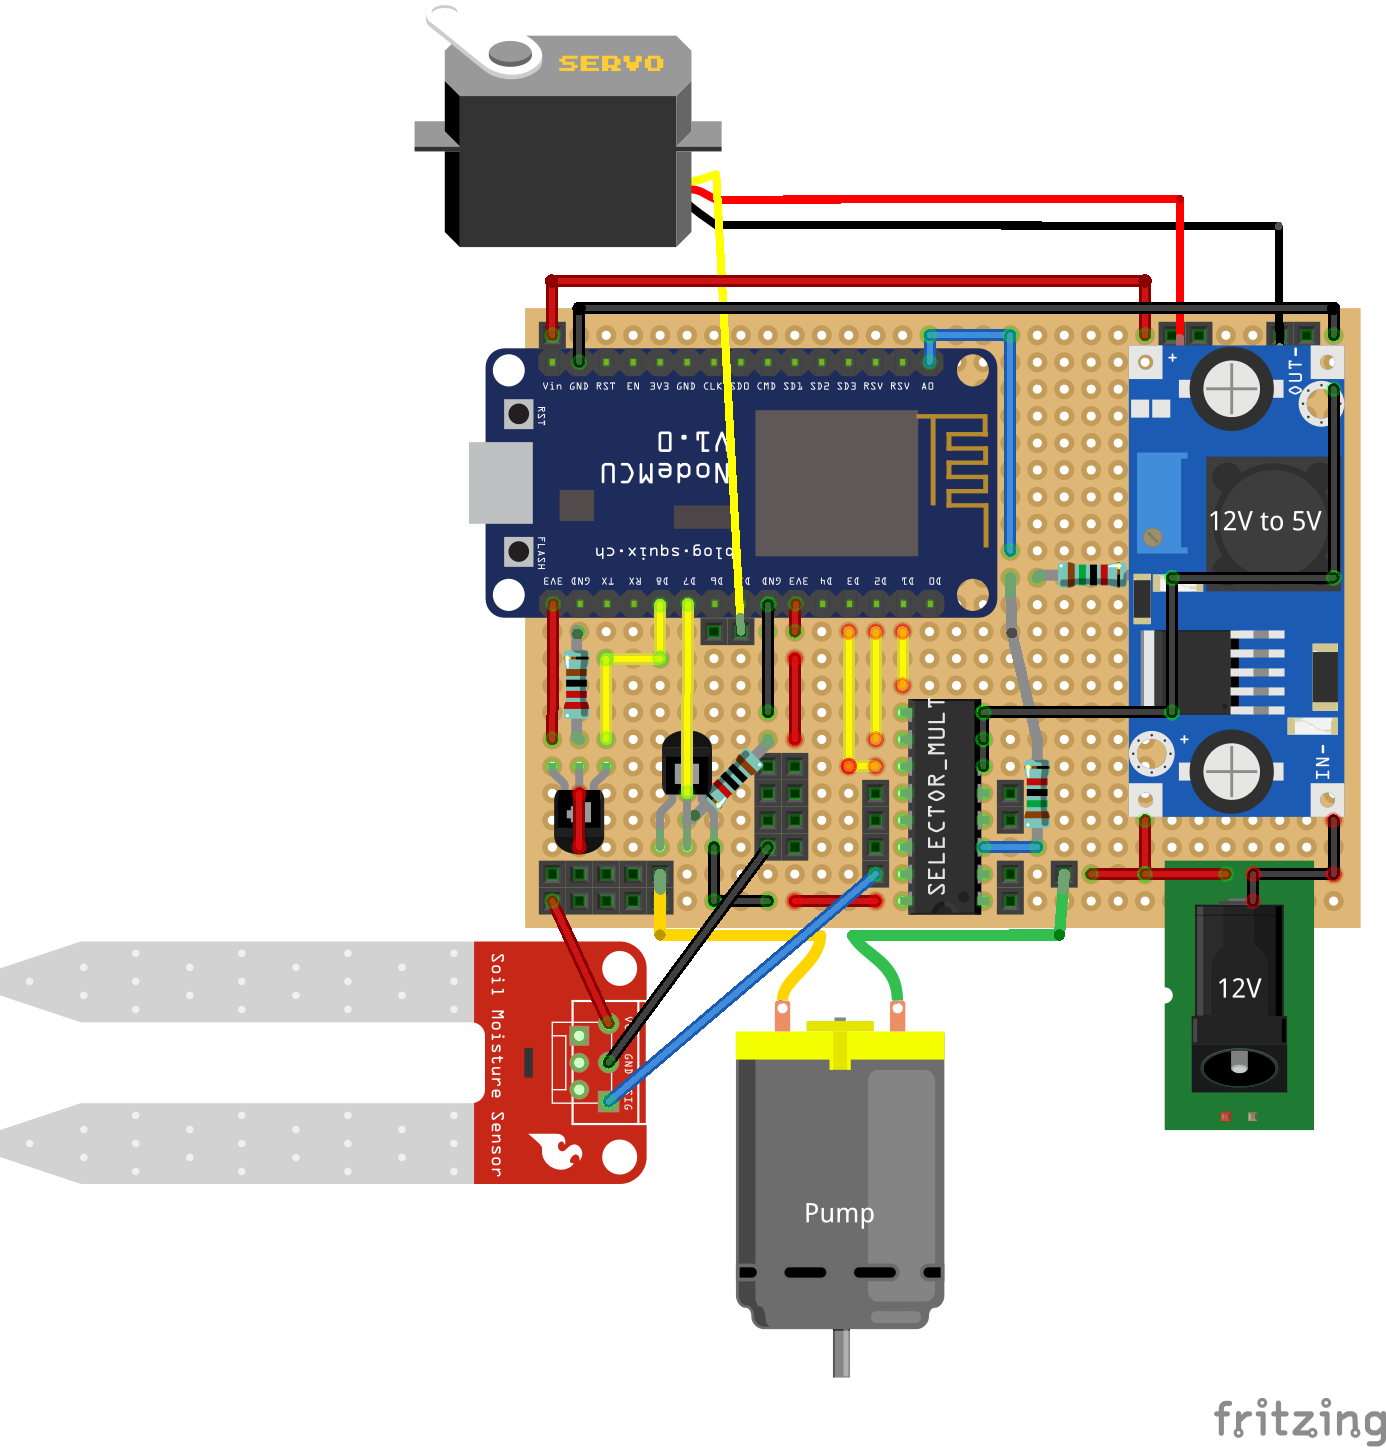
\includegraphics[width=0.8\linewidth]{Pictures/platinenlayout}
        \caption{Platinenlayout der Hardwarekomponenten}
        \label{fig:platinenlayout}
    \end{figure}
    \subsubsection{Installation / Ausführung}
    
    \paragraph*{Voraussetzung}
    \begin{itemize}
        \item Installierte Arduino IDE
        \item Treiber für den NodeMCU 1.0
    \end{itemize}

    \paragraph*{Installation}\mbox{}\\
    Zuerst muss die Unterstützung für den NodeMCU durch die Arduino IDE installiert werden. Dazu unter \textit{Werkzeuge --> Board --> Boardverwalter} das Paket \textit{esp8266} von der \textit{ESP8266 Community} installiert werden sowie unter \textit{Werkzeuge --> Board} das Board \textit{NodeMCU 1.0} ausgewählt werden. Nachdem Verbinden des Boards muss der richtige Port unter \textit{Werkzeuge --> Port} ausgewählt werden. Weiter muss die Library \textit{PubSubClient} von \textit{Nick O'Leary} mittels \textit{Sketch --> Bibliothek einbinden --> Bibliotheken verwalten} installiert werden.
    
    Anschließend müssen noch die Controller-ID sowie die Verbindungseinstellungen konfiguriert werden:
    \begin{itemize}
        \item ID.h\\
        ID des Controllers, welche ebenfalls auf dem Server hinterlegt sein muss
        \item WifiConfig.h\\
        Name und Passwort des Wlans mit dem sich der Controller verbinden soll
        \item MqttConfig.h\\
        Verbindungsdetails für den MQTT-Broker
    \end{itemize}

    Anschließend kann der Code mittels des Buttons \textit{Hochladen} auf den Controller übertragen werden. Damit sowohl Pumpe als auch Servo-Motor funktionieren, muss die Platine mit einer 12V-Stromversorgung verbunden sein.
    
     
    